

\subsection{Iteración 2}

En esta sección se van a llevar a cabo pruebas con usuarios reales para analizar la eficacia y usabilidad del sistema desarrollado. Para esto se ha creado un cuestionario del que se hablará a continuación y se ha presentado a los usuarios con el juego para que realicen 5 pruebas cada uno. Los usuarios varían tanto en edad y sexo, como en conocimientos tecnológicos previos para obtener información más amplia.



\subsubsection{Cuestionario}

Para evaluar la usabilidad del sistema se ha optado por utilizar un cuestionario SUS (System Usability Scale) ya que se trata de un sistema estándar el el desarrollo de software para medir la calidad y usabilidad de un programa. Se entiende como usabilidad la capacidad del programa para ser comprendido y utilizado por una persona.

Esta es una métrica fundamental en este proyecto, ya que un sistema poco usable, aunque tuviera una gran efectividad, reduciría drásticamente su calidad al dificultar su uso y entendimiento para el usuario. Por desgracia, para este proyecto no se dispone de los conocimientos, profesionales, tiempo ni usuarios para poder hacer un buen análisis de su efectividad y eficacia como sistema contra el deterioro cognitivo leve o para el entrenamiento cognitivo en general.

Por estos motivo, para el ámbito de este proyecto, solo se va a estudiar la usabilidad y todas las opiniones o pensamientos que ofrezcan los participantes.

El cuestionario que se les ha presentado a los usuarios se encuentra detallado en el apéndice \textbf{Cuestionarios} (\ref{sec:apendice:Custionarios}). Se trata de un cuestionario estándar con 10 preguntas a las que se responde con un número entre el 1 y el 5 indicando el grado con el que los usuarios están o no de acuerdo con el enunciado, significando un 1 que están totalmente en desacuerdo, y un 5 que están totalmente de acuerdo. Este método de evaluación se conoce como la escala Linkert y permite obtener un resultado más preciso de las opiniones del usuario al ofrecerle poder expresar su grado exacto de concordancia con los enunciados, además de permitir cuantificar numéricamente las respuestas de cada usuario para posterior análisis \cite{DES_5_2_linkert}.


El cuestionario, siguiendo el estándar SUS contiene diez enunciados, cinco de los cuales son positivos y el resto negativos. Dichos enunciados se presentan de forma alterna para hacer el test lo más homogéneo posible y limitar el sesgo. Una vez respondidos los cuestionarios, se puede obtener una calificación entre 0 y 100 puntos mediante una fórmula matemática sencilla:

\begin{itemize}
	\item{Sumar los resultados de los enunciados positivos y restar 5.}
	
	\item{Restar a 25 la suma de los enunciados negativos.}
	
	\item{Por último, sumar los dos números anteriores y multiplicar el resultado por 2,5.}
	
\end{itemize}

De esta forma, se obtiene un resultado que puede puntuar la usabilidad del sistema según el usuario. Aunque la escala es lineal entre 0 y 100, solo se considera que un sistema tiene una buena usabilidad si su puntuación en el test SUS supera los 68 puntos.

\subsubsection{Pruebas}

Las pruebas que se han realizado consisten en una sesión de juego de una duración de 5 minutos aproximandamente. Las personas seleccionadas para llevar a cabo estas pruebas pertenecen a distintos grupos de edad, conocimientos tecnológicos y familiaridad con la realidad virtual.

Un total de seis personas han prestado su ayuda para este estudio, las cuales se pueden clasificar de la siguiente forma:

\begin{itemize}
	\item{\textbf{Edad}. Tres personas tienen entre 20 y 30 años. Otras 3 tienen más de 60 años.}
	
	\item{\textbf{Conocimientos tecnológicos}. Cuatro personas tienen al menos conocimientos tecnológicos básicos, dos de las cuales tienen conocimientos avanzados. Otras dos personas no tienen conocimientos tecnológicos.}
	
	\item{\textbf{Familiaridad RV}. Dos personas están familiarizadas con la realidad virtual por experiencias previas. Para otras cuatro personas, esta ha sido su primera experiencia en realidad virtual.}
	
\end{itemize}

A cada persona se le ha asignado una letra (de la A a la F) para diferenciarlos y proteger su identidad. Para ver como se distribuyen en concreto estas personas en los tres grupos anteriores, se ha creado la tabla de la figura \ref{fig:tablaPersonasLetras} en la que se pueden ver cada una de las personas encuestadas clasificadas en las tres categorías, según edad, conocimiento tecnológico y si están familiarizadas con la RV o no.


%\begin{figure}
%	\centering
%	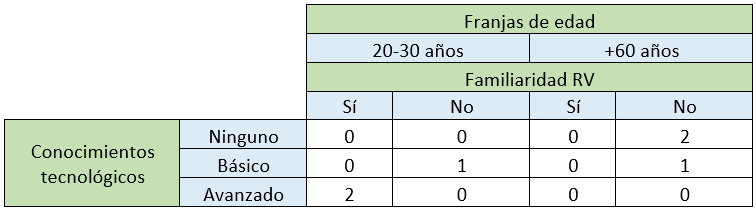
\includegraphics[width=0.7\textwidth]{04.Desarrollo/05.Entrega5/02.Iteracion5_2/00.Figuras/01.tabla_personas.png}
%	\caption{Número de personas encuestadas divididas por grupos de edad, conocimientos tecnológicos y familiaridad con la RV.}
%	\label{fig:tablaPersonas}
%\end{figure}


\begin{figure}
	\centering
	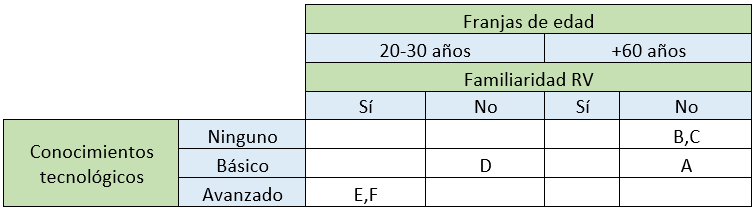
\includegraphics[width=0.7\textwidth]{04.Desarrollo/05.Entrega5/02.Iteracion5_2/00.Figuras/02.tabla_personas_letras.png}
	\caption{Personas encuestadas identificadas por letras y divididas por grupos de edad, conocimientos tecnológicos y familiaridad con la RV.}
	\label{fig:tablaPersonasLetras}
\end{figure}


A todas las personas se les ha dado una explicación de la motivación y objetivo del juego, así como de los controles y todo lo que necesitan saber para poder utilizar el juego. En todo momento durante las pruebas las personas han estado acompañadas y, en caso de ser necesario, aconsejadas sobre como actuar o avanzar en el juego.

Aunque el juego y las gafas de RV permiten el uso de forma completamente independiente, las pruebas se han realizado con un cable uniendo las gafas a un ordenador desde el que poder monitorizar lo que ve y hace el jugador, así como poder realizar grabaciones de vídeo para posterior estudio.


En el repositorio de Github en el que se encuentra este proyecto (\url{https://github.com/Eltrio723/TFG}), están disponibles algunos vídeos de las pruebas realizadas.


\subsubsection{Resultados}




\ref{sec:apendice:Custionarios:Resultados}








\subsubsection{Opinión profesional}











